%%%%%%%%%%%%%%%%%%%%%%%%%%%%%%%%%%%%%%%%%%%%%%%%%%%%%%%%%%%%%%%%%%
%%%%%%%% CPSC 66 SPRING 2021  REPORT %%%%%%%%%%%%%%%%%%%%%%%%
%%%%%%%% This template is modified from ICML 2014 %%%%%%%%%%%%%%%%
%%%%%%%%%%%%%%%%%%%%%%%%%%%%%%%%%%%%%%%%%%%%%%%%%%%%%%%%%%%%%%%%%%

\documentclass{article}

%include any external packages here.  This is similar to loading a
%library in python or C++

% use Times
\usepackage{times}
% For figures
\usepackage{graphicx}
\usepackage{subfigure}

% For citations
\usepackage{natbib}

% For algorithms and pseudocode
\usepackage{algorithm}
\usepackage{algorithmic}

%Adds hyperlinks to your citations automatically
\usepackage{hyperref}

% Packages hyperref and algorithmic misbehave sometimes.  We can fix
% this with the following command.
\newcommand{\theHalgorithm}{\arabic{algorithm}}
\usepackage[rightcaption]{sidecap}
\usepackage[accepted]{icml2014}


% If your title is long (below), use this command to also provide
% short version.  This will go on the top of every page
\icmltitlerunning{Final Report}

\begin{document}

\twocolumn[ %use two column if you need a text to span across the whole page
\icmltitle{ CPSC 66 Final Report: \\ % \\ force a new line
Environmental Justice: Using Machine Learning Models to Classify Communities with High Rates of Asthma }

\icmlauthor{Alexandara Baratta}{abaratt1@swarthmore.edu}
\icmlauthor{Muhammad Ghazi Randhawa}{mrandha11@swarthmore.edu}
\icmlauthor{Sidhika Tripathee}{stripat1@swarthmore.edu}
\vskip 0.3in
]


 \begin{abstract}
Our project trains four machine learning models to classify communities that face high rates of asthma. We were more interested in which features determine higher rates of asthma rather than accuracy rates. We compiled a data set for 324 counties across 6 states containing variables of interest like the racial demographics and number of incinerators in the county. We hypothesized that counties with higher Black population percentages will have more waste facilities in their communities and will have higher rates of asthma. We developed two sets of labels: one set had four labels while the second set of labels had two labels. After performing hyper tuning using grid search and validation curves on each of the models, we looked at the feature importance. The two label data gave us higher accuracy for each model than the four label data. Some of the two-label data trained models gave starkly higher importance to the racial demographics of counties (specifically communities of color) in determining whether a community has a higher risk. We think expanding the data set to include a very representative sample of USA would give even more valid findings. 
\end{abstract} 
\section{Introduction} 
\label{introduction} 
Environmental justice is described as a movement advocating for active and equal involvement of communities of all peoples as equal chaperons and beneficiaries of environmental conservation and rejuvenation. In the context of the United States, communities of color and minorities have been subjected to more than their right share of environmental damages. Historically, zoning laws have enabled certain communities to effectively outsource their waste disposals to less affluent communities, specifically Black and low income neighborhoods. An example portraying this injustice can be seen in Chester, Pennsylvania. Despite having a population of only 33,972, the city of Chester’s trash incinerator is the second largest incinerator in the country accumulating waste from not only Pennsylvania, but also New York, New Jersey, and Maryland. According to 2010 Census Data, the majority of Chester’s population is Black consisting of 20.6\% white, 68.9\% black, 0.3\% Native American, 0.6\% Asian, and 3.7\% mixed race. Furthermore, the median household income was \$32,403 and 31.4\% of the population is living in poverty. The pattern of unjust environmental impacts on low income communities of color is not only seen through waste disposal, but also through the locations of heavily polluting sites like fossil fuel power plants. Both waste facilities and power plants cause higher levels of air pollution leading to greater prevalence of health issues in these communities. 
 
USA’s Clean Air Act of 1963 along with its revisions in subsequent decades make it the responsibility of the Environmental Protection Agency to maintain air quality in pursuit of public health. Another relevant law is the Presidential Executive Order 12898 which implores executive agencies to consider environmental justice concerns when making decisions, but it does not mandate the agencies to base their decisions on these concerns. Furthermore, the agencies have an unwillingness to remediate these environmental justice grievances because legally environmental injustice can be difficult to be proved. The only permanent solution is to increase public awareness in an attempt to generate pressure on the regulatory agencies to enforce their mandate, provide borderline irrefutable evidence on the problem and to generate pressure onto corporations involved to follow these regulations. As such, a model that is able to accurately classify whether a community is at heightened risk of air pollution related health problems and demonstrate which factors most affect at-risk communities can help highlight this problem. 
 
The motivating question for this project was whether we could train machine learning models to predict if a community is at higher risk of asthma and identify which factors contribute most significantly to the higher rates within a community. The models that we considered for this project were Decision Trees, Random Forests, Logistic Regression Classifier, and Support Vector Machines (SVMs). We would have liked to train more models if it were not for time constraints. Our Approach section describes  the theory behind the four models in detail. Our experimental results section expand on our experimental methodology that we employed for training these four models and discuss the results we obtained for each model. Next, our paper states the social implications of this project. Our paper will end with a conclusion and suggestions to expand the project.

\section{Methods}
\label{methods}
The aim of our project was to train models that are accurately able to predict if a test example of a county is at a higher risk of asthma compared to the average found in the training data. We believe that an accurate model would be able to help us determine which features of a community create higher rates of asthma. For each of the four models we used, we hypertuned certain parameters for the model by the use of GridSearch and validation curves on certain parameters of interest for each model. We will describe these two methods and then the particular models each.

\subsection{Hyper tuning: Pipeline}
\label{Pipeline}
A pipeline allows us to automate the machine learning workflow by enabling data to be transformed and correlated with a model. We used the Pipeline() function from the scikit-learn library to create a pipeline for each of the models. For each of the pipelines, we used StandardScalar() to standardize the data, computed dimensional reduction using Principal Component Analysis (PCA) and created an object for the appropriate classifier. We then uses the pipeline object to compute GridSearch. 

\subsection{Hyper tuning: Grid Search}
\label{Grid Search}
A grid search automatically iterates through a determined range of values for parameters of the model and outputs the combination of parameters that yield the highest accuracy. It determines the accuracy for each combination through cross validation where the number of folds can be determined. We used the GridSearchCV() function from the scikit-learn library to iterate through a range of variables for parameters of interest. We had to sometimes limit our parameters for grid search due to time and resource constraints. We used a 4-fold cross validation for all of our models. 

\subsection{Hyper tuning: Validation Curves}
\label{Validation curves}
For each of the models, we ran validation curves for the most important parameter to determine the amount of over fitting and under fitting. We used the validation curve function of scikit-learn to achieve that purpose.

\subsection{Decision Trees}
\label{decision trees}
A decision tree is a non-parametric supervised learning method used for classification and regression. We used its classification implementation from scikit-learn library. A decision tree uses a tree-based approach where each node represents a test on a particular feature with each of its children nodes representing a particular outcome of the test, and each leaf of the tree represents a particular class label of the example. It is structured on the principle of information gain and entropy from information theory. Entropy is defined as the randomness in a data set while information gain of a feature is determined to be the decrease in entropy when the data is divided into at least two groups based upon the feature. The following two equations are used for the task:
\begin{center}
$Entropy:$
    $H(X) = -\sum p(X)\log p(X)\ $ \newline
    and $\newline
Information\ Gain\; I(X,Y)\equiv H(X)-H(X|Y)\
$ 
\end{center}
where $X$ is a feature, $x$ is a particular value of $X$ and Y is a label from the data. 
\newline\newline
As such, the decision tree algorithm is structured such that the feature with the most information gain in the training data set is tested upon first. Decision trees are better at working with discrete features than continuous features. Even though our data consisted of continuous features, we decided to use Decision Trees because they can be very easy to visualize. The parameters we hyper tuned upon were: ccp-alpha, criterion, class weight and max depth. We ran validation curves with the parameter of max-depth.

\subsection{Random Forests}
\label{random forests}
Random forest classifier is a supervised learning model that tries to overcome the high bias problem with decision trees. It achieves this with a bagging ensemble implementation with decision trees and its final classifier is determined by voting from the constituent decision trees. Bagging feature reduces bias in the construction of each member decision tree by selecting only a certain number of features for each decision tree to determine the label. The parameters we used for GridsearchCV() for Random Forests were bootstrap and number of estimators. We also ran validation curves on the number of estimators.

\subsection{Logistic Regression}
\label{logistic regression}
Logistic regression is a form of regression that performs classification using the logistic (also known as sigmoid) function. Unlike linear regression, it assumes that the data follows a sigmoid function and the only two possible values have to choose between a label of 0 or 1. Given data for a testing example, logistic regression determines the probability of that being the label 1. If it is above a certain threshold, the label assigned is 1 and if it is below that threshold, it assigns a label of 0. We performed GridSearchCV() of logistic regression over the hyperparameter C and also ran validation curves on C. 

\subsection{Support Vector Machines}
\label{support vector machines}

Support Vector Machines (SVMs) is a classification algorithm that can do binary classification. For a given set of training data, the algorithm tries to find the hyper plane that is able to maximize the margin for both the data sets. This means that it is able to maximize the distance of the hyper plane from the closest member of both data groups. We ran GridSearchCV() on SVMs for C, gamma, and kernel. We did ran validation curves for the gamma variable.

\section{Experiments and Results}
\label{results}

\subsection{Data set Creation}
\label{dataset generation}

We generated our own data set for this project collecting 324 county data entries from six US states including New York, New Jersey, North Dakota, Arkansas, West Virginia, and California. For each county of every state, we used various databases to collect information about the county population, racial demographics, number of waste facility locations, PM2.5 concentrations, and asthma rates as the label. After creating our data set, we considered the distribution of asthma rates among our entries as seen in $Figure 1$: 

\begin{figure}[h]
\caption{Asthma Rates Histogram}
\centering
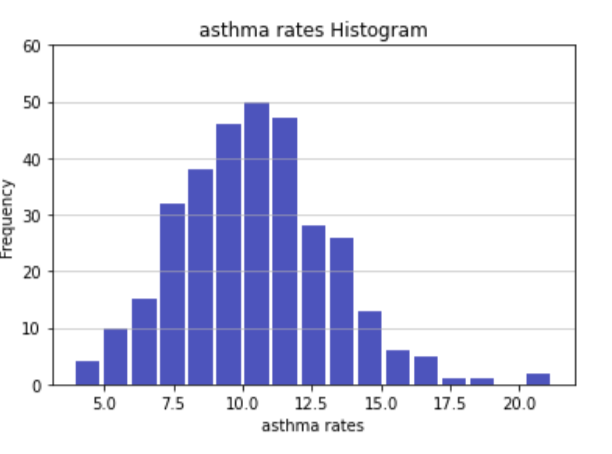
\includegraphics[scale=0.75]{Asthma Rates Histogram.png}
\end{figure}

We then created three limits within our data - the lower limit which was the mean minus the standard deviation, the medium limit which was the mean, and the upper limit which was the mean plus the standard deviation. From here, we separated our data into four categories: slightly lower risk which accounted for 112 asthma rates in our data that fell below the lower limit, lower risk which accounted for 52 asthma rates that fell between the lower limit and the medium limit, slightly higher risk which accounted for 107 asthma rates that fell between the medium limit and the upper limit, and finally higher risk which accounted for 53 asthma rates that fell above the upper limit. 

After reviewing the results of this method for labeling our data, we decided to shift our benchmarks and create only two classifications of asthma rates: lower risk and higher risk. The lower risk category accounted for data entries in which the asthma rates were below the mean + 0.5*standard deviation, whereas the higher risk category accounted for data entries in which the asthma rates were above this benchmark. After making this shift, we saw higher accuracy rates in our models since we made the classification task more simple and only focused on whether or not a specific community was at a higher risk of asthma or not. 

In both our data with four labels and with two labels, we used 4 fold cross validation in order to more efficiently train our models on the limited sized data set that we had. 

\subsection{Logistic Regression Results}
\label{logistic regression results}

When running logistic regression on our data with four labels the highest accuracy were we able to achieve after hyper-tuning parameters was 34.6\%  the C parameter at 0.01. In terms of feature importance, we saw that Native American population, number of waste facilities, other population, and white population had the highest  feature importance as shown in the following graph: 

\begin{figure}[h]
\caption{Four Class Logistic Regression Feature Importance}
\centering
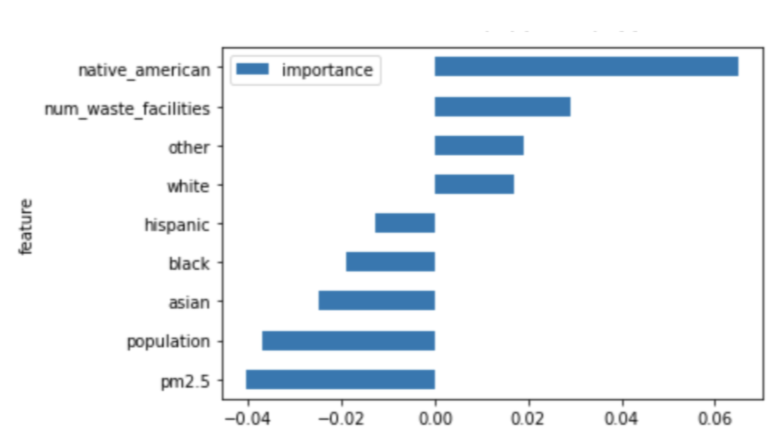
\includegraphics[scale=0.6]{4ClassLogReg.png}
\end{figure}

The accuracy of logistic regression increased to 75.38\% after running it on data with only two labels. In terms of feature importance, we got unexpected results. The features with the highest importance were Asian, PM2.5 concentration, population and Hispanic population. The Black population had the lowest feature importance as shown in the following graph:

\begin{figure}[h]
\caption{Two Class Logistic Regression Feature Importance}
\centering
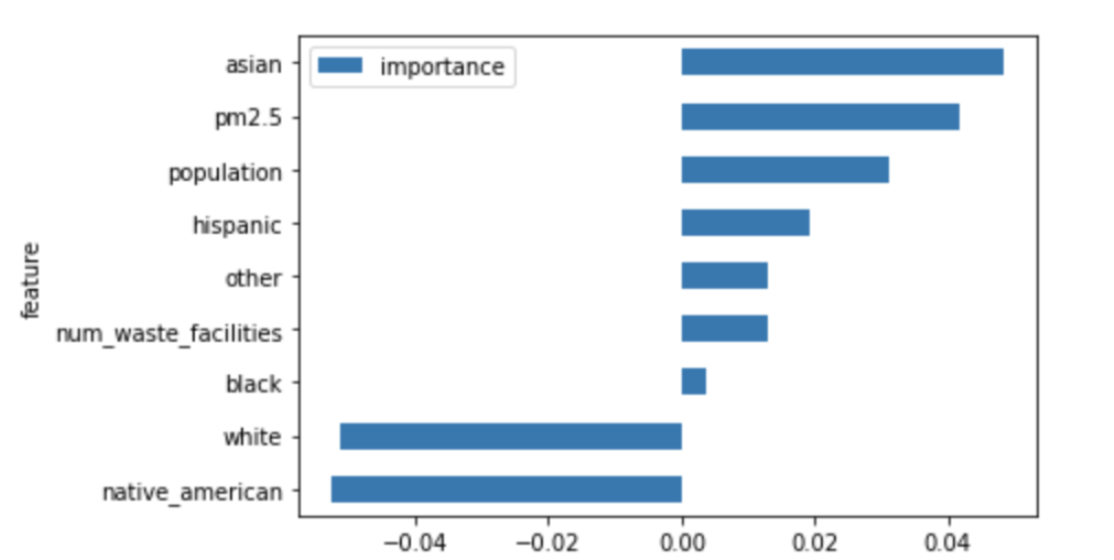
\includegraphics[scale=0.4]{2ClassLogReg.png}
\end{figure}

We believe that we got results that do not align with our hypothesis because logistic regression assumes linear distribution of our data which is not the case in this problem. We feel that the other three models we ran were better suited for our data. 

\subsection{Decision Tree Results}
\label{decision tree results}

When running decision trees on our data with 4 labels we achieved an accuracy of 38.5\% with a maximum depth of 5 to 6. In terms of feature importance, PM2.5 concentrations had the highest feature importance followed by population, other population and, Black population. Native American population, and number of waste facilities had  similar importance. White, Asian, and Hispanic racial demographics all had low feature importance as shown the following graph: 
\begin{figure}[h]
\caption{Four Class Decision Tree Feature Importance}
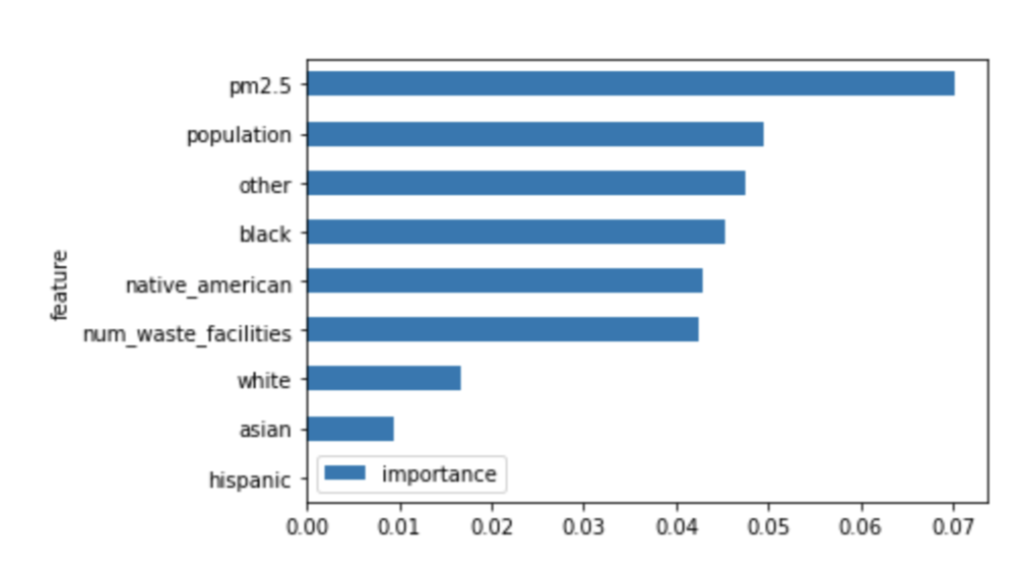
\includegraphics[scale=0.45]{4ClassDT.png}
\end{figure}

After running decision trees on our two class labeled data, the accuracy increased to 72.3\%. In terms of feature importance, we saw that Black, Hispanic, White, and PM2.5 concentrations were most important as shown in the following graph: 

\begin{figure}[h]
\caption{Two Class Decision Tree Feature Importance}
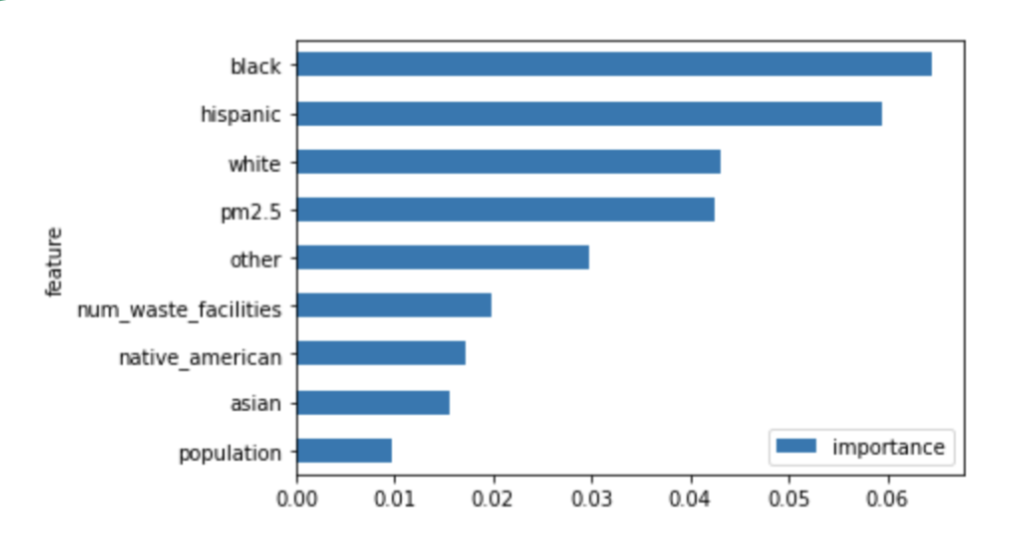
\includegraphics[scale=0.45]{2ClassDT.png}
\end{figure} 

The feature importance results of decision trees aligned more closely to our initial hypothesis, however the White population feature importance still was higher than expected. 

\subsection{Random Forest Results}
\label{random forest results}
Random Forests achieved a maximum accuracy of 39\% from GridSearchCV() for four labels data but their accuracy increased to 71\% when we switched to two labels. Going down from four labels to two labels increases our accuracy because it decreased the room for error in the final voting for the random forests. 

We drew two graphs for each model of random forest to determine the feature importance. The first one calculates and plots the mean and standard deviation of decrease in impurity for the random forest model across its member decision trees for each feature. However, this might not be the best measure of feature importance if the features have a high cardinality which our data does. As such, we drew mean and standard deviation of permutation feature importance for the two random forest models as well. Permutation feature importance measures the increase in the prediction error of the model after we permuted the feature's values, which breaks the relationship between the feature and the true outcome. As such, shuffling the values of a feature that was very important for the model would cause the prediction error of the model to increase more than the increase in prediction error of the model caused by a shuffle for a feature that was not that important for the model. 

\begin{figure}[h]
\caption{Four Class Random Forest Feature Importance}
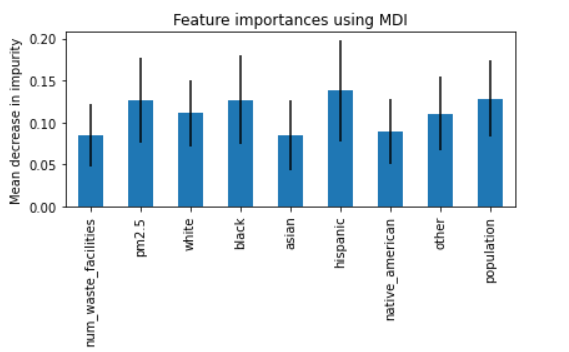
\includegraphics[scale=0.45]{MDI1.PNG}
\end{figure}

\begin{figure}[h]
\caption{Two Class Random Forest Feature Importance} 
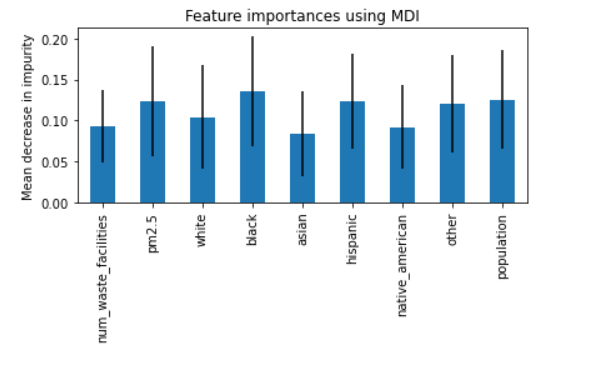
\includegraphics[scale=0.45]{MDI2.PNG}
\end{figure}


We can see that for the four label model using the MDI method, the most important feature was the proportion of latino community in the county and the proportion of the white community had similar importance as rest of the variables. However, the MDI for the two label data shows that most important feature was the proportion of black community in the county and the MDI for the proportion of white community in the county had a significant less mean and standard deviation for MDI.

\begin{figure}[h]
\caption{Four Class RF Feature Importance by permutation}
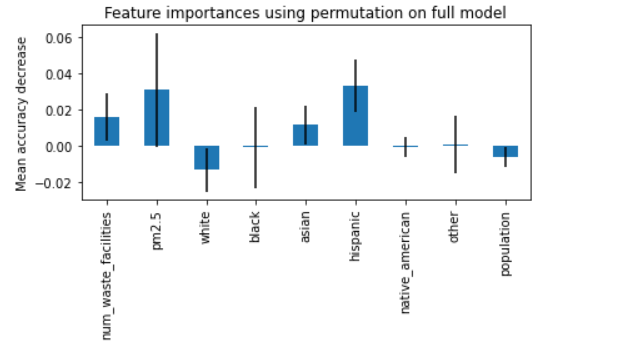
\includegraphics[scale=0.45]{featimprf1.PNG}
\end{figure}

\begin{figure}[h]
\caption{Four Class RF Feature Importance by permutation}
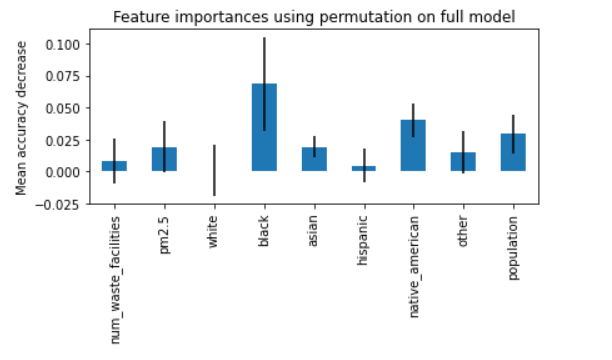
\includegraphics[scale=0.45]{featimprf2.PNG}
\end{figure}

The permutation feature importance mean and standard deviation graphs show us that the most important feature was pm 2.5 concentration in the county. The permutation graph for the 2 label data shows us that the most important feature for the random forest was Black population at significantly higher of a weight than any other feature. As such, we think the the Random Forest model with 2 labels' feature importance best aligns  with our hypothesis.


\subsection{Support Vector Machines Results}
\label{SVM results}

Support Vector Machines (SVMs) gave the highest accuracy with both four labeled data and two labeled data. When we ran SVMs on our four labeled data, we achieved an accuracy of 42\% with a linear kernel, the C parameters set to 1000, and gamma as 0.1. In terms of feature importance, however, we got unexpected results. The White racial demographic had the highest feature importance followed by Black, Asian, and Native American. PM2.5 concentration and number of waste facility locations both had low feature importance as shown in $Figure$ 10: 

\begin{figure}[h]
\caption{Four Class SVMs Feature Importance}
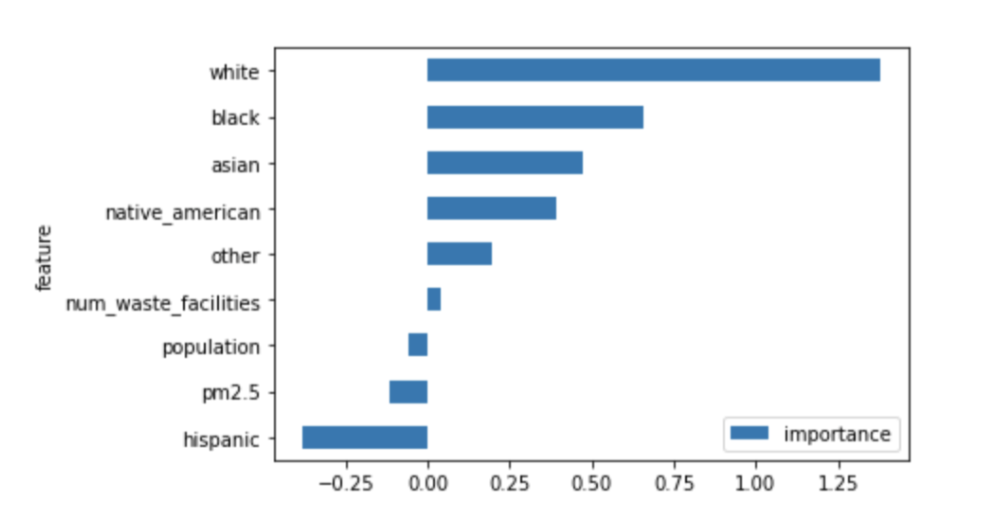
\includegraphics[scale=0.45]{4ClassSVM.png}
\end{figure}

After running SVMs on our two labeled data, our accuracy increased to 71.3\% with only pm2.5 having positive feature importance as seen in $Figure$ 11: 

\begin{figure}[h]
\caption{Two Class SVMs Feature Importance}
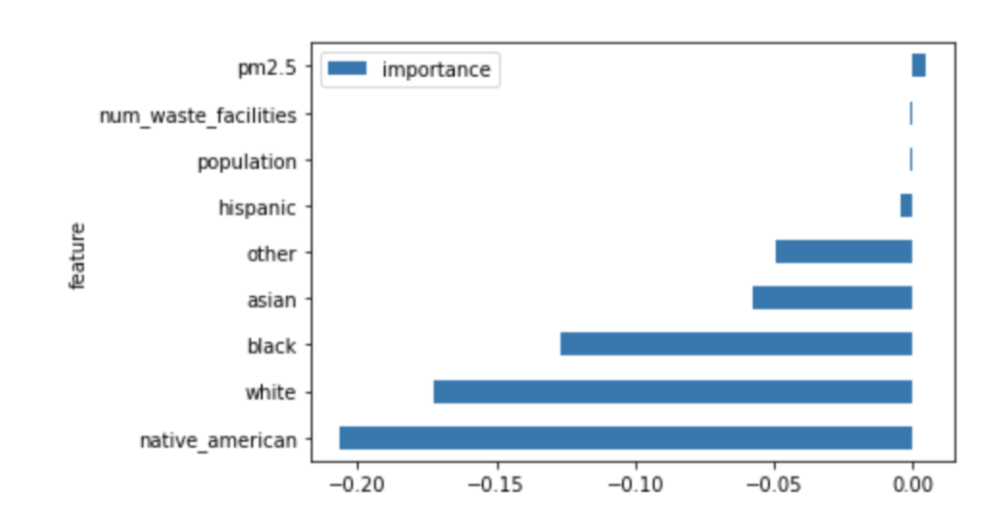
\includegraphics[scale=0.45]{2ClassSVM.png}
\end{figure} 

Although SVMs had the highest accuracy, the feature importance results do not really align with our hypothesis. This demonstrates that not all models are best at representing data even if the accuracy rates are high. 

\section{Conclusions}
\label{conclusion}

For our model consisting of two classifications of labels: lower risk and higher risk, both the Decision Tree Model and Random Forest Model showed that the Black racial demographic was the feature with the greatest importance in determining the asthma risk within a community. All of our models also suggested that PM2.5 concentration was in the top four most important features in determining the risk of a community. Although these results align with our hypothesis, we believe that in order to develop more consistent and and comprehensive results we need a larger data-set. At this time, we feel we are unable to make any significant conclusions based on our results.   

\subsection{Future Directions}
\label{Future Directions}

With more time, we would like to expand our data-set to include county data from every state in the country. We also would like to add additional features such as population density, average income rates, poverty levels and car ownership rates in order to explore how significantly other factors contribute to asthma rates within a community. We believe that with more data we could achieve higher accuracy on the models that we ran and perhaps feature importance would also become more consistent among models. We also feel it would be worthwhile to run our data on other models such as Neural Networks and Naive Bayes to determine if they are better suited for classifying the information. 

\subsection{Social Implications}
\label{social implications}

If we could further develop this project in order to produce results that align even more consistently with our hypothesis, we could generate specific evidence of environmental injustice within our country. The main people who may benefit from this work are the marginalized communities that are currently at higher risk of asthma or other health related conditions as a result of the unjust placement of waste facilities and heavily polluting sites. The conclusions we draw from this model can we used as supporting evidence towards policy makers that hopefully inspires action and accountability. 

Our models' implications are also very important for court proceedings in environmental justice cases. Since the Executive order on Environmental Justice does not make it mandatory for federal agencies to enforce it, courts often are the last resort in action against environmental injustices. Our models can be used as evidence of environmental justice problems concerning air pollution in USA because many of the models highlight that the proportions of minority communities in counties do determine the incidence of above average rates of asthma. 

An example of how our data can be used an evidence as well as educate the public is through a map displaying our results. Sidhika created the map below for her GIS class which used our data set. She focused on California and created a new feature combining all the non-white populations to starkly display environmental racism. The map  displays people of color populations with waste facilities frequency and asthma rates. From this map, we can see that waste facilities are placed in communities of people of color which correlates to higher asthma rates. 

\begin{figure}[h]
\caption{Map of Populations of Color in California and the correlation of Asthma Rates and Waste Facilities}
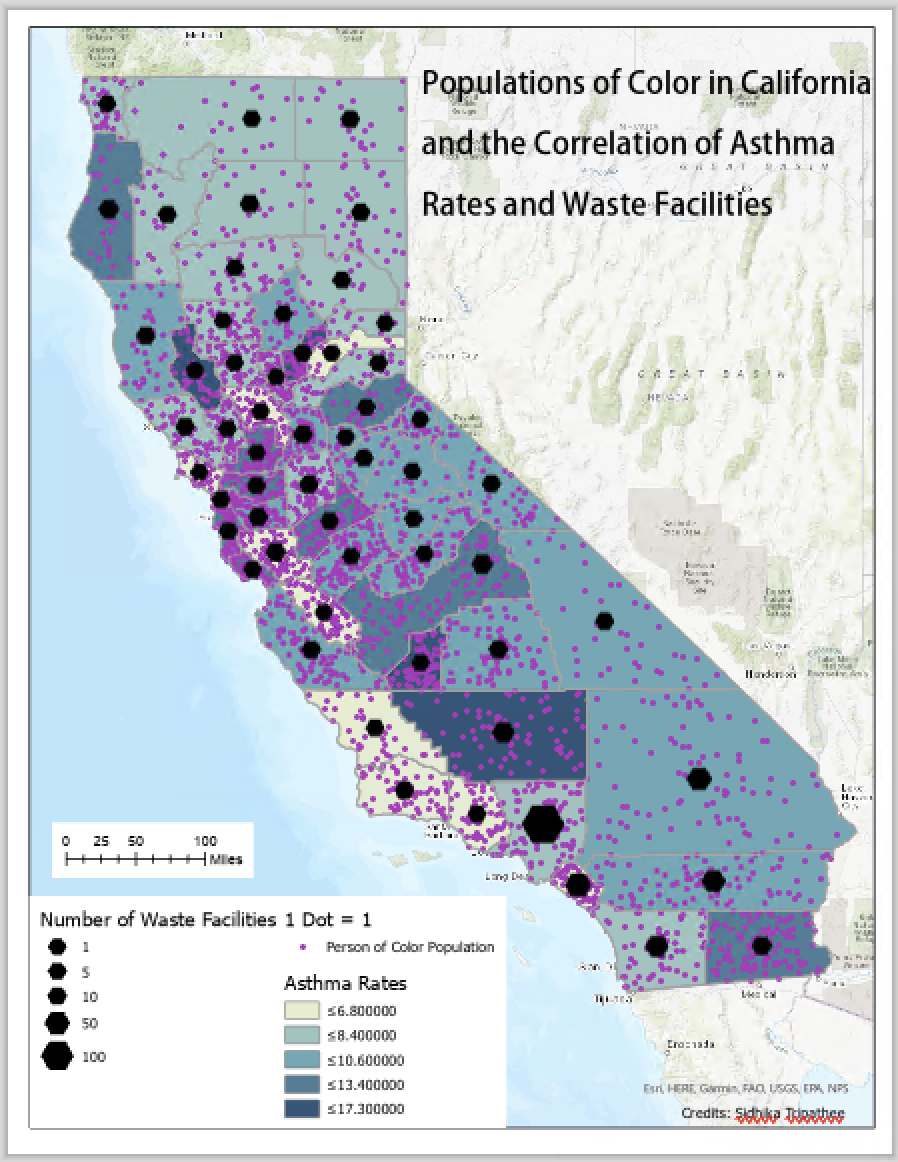
\includegraphics[scale=0.50]{Map.png}
\end{figure}

\section*{Acknowledgments}

Thank you to friends and family members who supported us through the difficult collection of the data set and even helped us out a little with the tedious task. Thank you to the professors for helping and guiding us throughout the span of this project.

% In the unusual situation where you want a paper to appear in the
% references without citing it in the main text, use \nocite
\nocite{EPA}
\nocite{cali}
\nocite{census}
\nocite{facilities}

\bibliography{references}
\bibliographystyle{icml2014}

\end{document}


% This document was modified from the file originally made available by
% Pat Langley and Andrea Danyluk for ICML-2K. This version was
% created by Lise Getoor and Tobias Scheffer, it was slightly modified
% from the 2010 version by Thorsten Joachims & Johannes Fuernkranz,
% slightly modified from the 2009 version by Kiri Wagstaff and
% Sam Roweis's 2008 version, which is slightly modified from
% Prasad Tadepalli's 2007 version which is a lightly
% changed version of the previous year's version by Andrew Moore,
% which was in turn edited from those of Kristian Kersting and
% Codrina Lauth. Alex Smola contributed to the algorithmic style files.
